\documentclass[9pt,twocolumn,twoside]{pnas-new}

% Use the lineno option to display guide line numbers if required.
% Note that the use of elements such as single-column equations
% may affect the guide line number alignment.


\usepackage[T1]{fontenc}
\usepackage[utf8]{inputenc}

% tightlist command for lists without linebreak
\providecommand{\tightlist}{%
  \setlength{\itemsep}{0pt}\setlength{\parskip}{0pt}}


% Pandoc citation processing
%From Pandoc 3.1.8
% definitions for citeproc citations
\NewDocumentCommand\citeproctext{}{}
\NewDocumentCommand\citeproc{mm}{%
  \begingroup\def\citeproctext{#2}\cite{#1}\endgroup}
\makeatletter
 % allow citations to break across lines
 \let\@cite@ofmt\@firstofone
 % avoid brackets around text for \cite:

 \def\@biblabel#1{}
 \def\@cite#1#2{{#1\if@tempswa , #2\fi}}
\makeatother
\newlength{\cslhangindent}
\setlength{\cslhangindent}{1.5em}
\newlength{\csllabelwidth}
\setlength{\csllabelwidth}{3em}
\newenvironment{CSLReferences}[2] % #1 hanging-indent, #2 entry-spacing
 {\begin{list}{}{%
  \setlength{\itemindent}{0pt}
  \setlength{\leftmargin}{0pt}
  \setlength{\parsep}{0pt}
   \normalfont\sffamily\fontsize{6}{8}\selectfont
    \labelsep2.8pt
   \renewcommand\newblock{\hskip .11em \@plus.33em \@minus.07em}
  % turn on hanging indent if param 1 is 1
  \ifodd #1
   \setlength{\leftmargin}{\cslhangindent}
   \setlength{\itemindent}{-1\cslhangindent}
  \fi
  % set entry spacing
  \setlength{\itemsep}{0.0pt}}}
 {\end{list}}
\usepackage{calc}
\newcommand{\CSLBlock}[1]{#1\hfill\break}
\newcommand{\CSLLeftMargin}[1]{\parbox[t]{\csllabelwidth}{#1}}
\newcommand{\CSLRightInline}[1]{\parbox[t]{\linewidth - \csllabelwidth}{#1}\break}
\newcommand{\CSLIndent}[1]{\hspace{\cslhangindent}#1}

\usepackage{tikz}
\usetikzlibrary{angles,positioning,arrows.meta, quotes, shapes, shapes.geometric}
\usepackage{graphicx}
%\usepackage{emoji}
\usepackage{caption, subcaption}
\usepackage{booktabs}
\usepackage{longtable}
\usepackage{array}
\usepackage{multirow}
\usepackage{wrapfig}
\usepackage{float}
\usepackage{colortbl}
\usepackage{pdflscape}
\usepackage{tabu}
\usepackage{threeparttable}
\usepackage{threeparttablex}
\usepackage[normalem]{ulem}
\usepackage{makecell}
\usepackage{xcolor}

\templatetype{pnasresearcharticle}  % Choose template

\begin{document}
\title{Interaction structure constrains the emergence of conventions in
group communication}

\author[a,1]{Veronica Boyce}
\author[b]{Robert D. Hawkins}
\author[a,c]{Noah D. Goodman}
\author[a]{Michael C. Frank}

  \affil[a]{Psychology Department, Stanford University, Stanford, CA
94305}
  \affil[c]{Computer Science Department, Stanford University, Stanford,
CA 94305}
  \affil[b]{Psychology Department, University of Wisconsin -- Madison,
Madison, WI, 53715}


% Please give the surname of the lead author for the running footer
\leadauthor{Boyce}

% Please add here a significance statement to explain the relevance of your work
\significancestatement{Human linguistic communication is remarkably
versatile, from one-on-one conversations to large group chats on
messaging platforms. Yet existing empirical work has overwhelmingly
focused on one-on-one contexts, overlooking the factors that affect
real-world communication in larger groups. We address this gap using a
large-scale reference game task, examining how groups of varying sizes
and interaction structures coordinate on linguistic conventions for
novel objects. We found effective and robust communication across
multiple settings, but larger (6-person) groups were more sensitive to
differences in group structure and communication channels. Our results
suggest that ``thicker'' communication channels - where group members
provide more feedback to one another - can result in better
communication in larger groups.}


\authorcontributions{We report CRediT taxonomy contributions as follows:
All authors did conceptualization and methodology. VB did data curation,
formal analysis, investigation, visualization, and writing -- original
draft. VB and RDH did software. RDH, NDG, and MCF did writing --
editing. MCF and NDG did funding. MCF did supervision.}



\correspondingauthor{\textsuperscript{1} To whom correspondence should
be addressed. E-mail:
\href{mailto:vboyce@stanford.edu}{\nolinkurl{vboyce@stanford.edu}}}

% Keywords are not mandatory, but authors are strongly encouraged to provide them. If provided, please include two to five keywords, separated by the pipe symbol, e.g:
 \keywords{  Communication |  Psycholinguistics |  Reference
games |  Convention formation |  large-scale online experiment  } 

\begin{abstract}
Real-world communication frequently requires language producers to
address more than one comprehender at once, yet most psycholinguistic
research focuses on one-on-one communication. As the audience size
grows, interlocuters face new challenges that do not arise in dyads.
They must consider multiple perspectives and weigh multiple sources of
feedback to build shared understanding. Here, we ask which properties of
the group's \emph{interaction structure} facilitate successful
communication. We used a repeated reference game paradigm in which
directors instructed between one and five matchers to choose specific
targets out of a set of abstract figures. Across 313 games (\(N=1,319\)
participants), we manipulated several key constraints on the group's
interaction, including the amount of feedback that matchers could give
to directors and the availability of peer interaction between matchers.
Across groups of different sizes and interaction constraints, describers
produced increasingly efficient utterances and matchers made
increasingly accurate selections. Critically, however, we found that
smaller groups and groups with less-constrained interaction structures
(``thick channels'') showed stronger convergence to group-specific
conventions than large groups with constrained interaction structures
(``thin channels''), which struggled with convention formation. Overall,
these results shed new light on the core structural factors that enable
communication to thrive in larger groups.
\end{abstract}

\dates{This manuscript was compiled on \today}
\doi{\url{www.pnas.org/cgi/doi/10.1073/pnas.XXXXXXXXXX}}



% Optional adjustment to line up main text (after abstract) of first page with line numbers, when using both lineno and twocolumn options.
% You should only change this length when you've finalised the article contents.




\maketitle
\thispagestyle{firststyle}
\ifthenelse{\boolean{shortarticle}}{\ifthenelse{\boolean{singlecolumn}}{\abscontentformatted}{\abscontent}}{}

\firstpage[11]{3}
% If your first paragraph (i.e. with the \dropcap) contains a list environment (quote, quotation, theorem, definition, enumerate, itemize...), the line after the list may have some extra indentation. If this is the case, add \parshape=0 to the end of the list environment.

\acknow{We thank the LangCog Lab, Saxelab, CAMP 5, HSP 2023, and Cogsci
2022 audiences for helpful feedback on this work. Experiment 1 was
previously reported in Proceedings of the Annual Meeting of the
Cognitive Science Society 44 (2022). This work was supported by a
Hoffman-Yee Grant from the Stanford Institute for Human-Centered AI.}

%Pre-print status: this work is on the pre-print server PsyArxiv at
%\url{https://osf.io/preprints/psyarxiv/a3wfy} under a CC-BY license.

%Classification: Social Sciences -\textgreater{} Psychological and
%Cognitive Sciences

Much of human social life revolves around communication in groups. At
school, teachers address large classrooms of children (1); at home, we
chat with groups of friends and family members over dinner (2); and at
work, we attend meetings with colleagues and managers (3, 4). Such
settings present considerable challenges that do not arise in the purely
two-party (dyadic) settings typically studied in psychology (5--7). For
example, producers need to account for the fact that different
comprehenders in the group may have different mental states or levels of
background understanding (8--13), while comprehenders must account for
the fact that utterances are not necessarily tailored to them (14--20).
What enables producers and comprehenders to nevertheless overcome these
challenges and navigate multi-party settings with relative ease?

One promising set of hypotheses centers on the group's \emph{interaction
structure}, the set of constraints placed on the group's shared
communication channel. Many different aspects of interaction structure
have been implicated in the effectiveness of dyadic communication,
including the availability and quality of concurrent feedback (21--23),
the bandwidth of the communication modality (24, 25), and the group's
access to a shared workspace (26, 27). Yet larger groups introduce
qualitatively different dimensions of interaction structure, leading to
a large but often inconsistent body of findings even for these
well-understood factors (28, 29). While communication is generally
expected to deteriorate as groups get larger (30, 31), the structural
``thickness'' of the feedback channel may slow such deterioration (32,
33).

In this paper, we develop an experimental paradigm for evaluating the
relative contribution of these factors: a \emph{multi-party repeated
reference game.} The ability to distinguish one particular entity from
other possible entities, known as \emph{reference}, is one of the most
primitive and ubiquitous functions of communication. Reference games
(34, 35) have been widely used to study dyadic communication under
controlled conditions in the lab. They provide a clear metric of
communicative effectiveness: how many words are required before a
matcher successfully chooses a target image from a context of
distractors? \emph{Repeated} reference games, where the same target
images appear multiple times in succession, were introduced to examine
how interlocutors establish shared reference in the absence of
conventional labels (36, 37). At the beginning of the game, long and
costly descriptions are typically required to succeed. A key finding,
however, is that dyads become increasingly efficient over the course of
interaction. Fewer words are required to achieve the same accuracy, but
referring expressions also become more impenetrable to outsiders (38,
39). The evolution of referring expressions over repetitions shows the
characteristic dynamics of conventions: \emph{stability}, or convergence
on labels within a group, and \emph{arbitrariness}, or divergence to
different across groups, suggesting that dyads leverage their shared
communication history to coordinate on expectations about how to label
the target images (40).

In principle, repeated reference games provide a strong
operationalization of communicative effectiveness for the problem of
multi-party communication: describers must simultaneously achieve shared
reference with multiple matchers. However, empirically studying
multi-party communication raises a number of difficulties in practice. A
much larger pool of participants must be recruited to achieve sufficient
power at the relevant unit of analysis -- the group -- spanning a very
high-dimensional space of possible parameter settings (41). We address
this problem by drawing on recent technical advances that have made it
newly possible to achieve such samples using interactive web-based
platforms (40, 42, 43). Repeated reference games in web-based platforms
have previously replicated earlier results from face-to-face studies,
although people produce fewer words in text modalities than oral
modalities (44). The text-based chat modalities arguably more closely
resemble the interfaces used by modern teams who increasingly
communicate through group text threads or popular platforms like Slack
or Discord.

We leverage our platform to explore effects of group size and
interaction channel thickness in a series of three experiments. While we
find that small groups reliably converge on group-specific ``shorthand''
regardless of the interaction structure, larger groups require thicker
channels -- richer conversational feedback among members -- to achieve
the same degree of coherence. Thus, increasing group size alone does not
impede communication; rather, larger groups may require stronger social
and linguistic cues to establish common ground among all members. More
broadly, our work suggests that studying communication in larger groups
is necessary to unveil critical aspects of interaction structure that
have not been evident in typical dyadic settings.

\begin{figure*}[t!]

{\centering 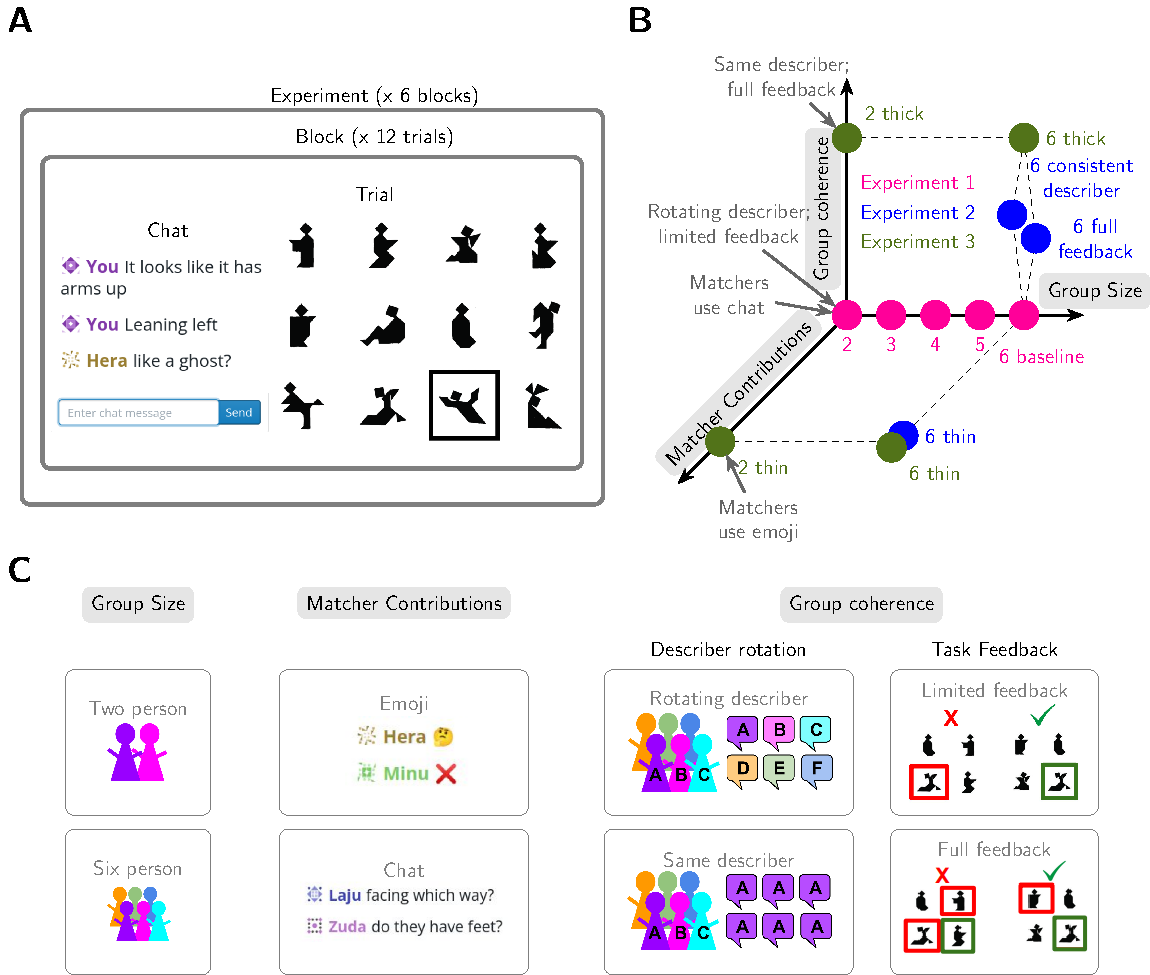
\includegraphics[width=1\linewidth]{expt-diagram4.pdf} 

}

\caption{(A) Participants played a repeated reference game in groups of size 2 to 6. On each trial, a describer described the target image to the group of matchers. Each image appeared once per block for six blocks. (B) Experiments varied along 3 dimensions: Group size, group coherence, and matcher contributions. (C) Experiment 1 (pink) varied group size from 2 to 6 players while holding group coherence and matcher contributions constant. Experiment 2 (blue) held group size constant at 6 and manipulated the other dimensions. Experiment 3 (green) tested 4 corners of the space, crossing group size (2 vs. 6 players) with the thickness of interaction structure (high vs. low coherence and matcher contributions).}
\end{figure*}

\section*{Results}\label{results}
\addcontentsline{toc}{section}{Results}

We recruited 1319 participants through Prolific, an online
crowd-sourcing platform. Participants were organized into 313 groups of
size two to six for a communication game (Figure 1A).
On each trial, everyone in the group was shown a gallery of 12 tangram
images (37, 44, 45). One player was designated the \emph{describer} and
the others were designated the \emph{matchers}. The describer was asked
to use a chat box interface to describe a privately indicated
\emph{target} image. After all matchers guessed which of the 12 images
was the target, they received task feedback and proceeded to the next
trial. The game consisted of 72 trials structured into 6 repetition
blocks, where each image appeared as the target exactly once per block.

We manipulated the interaction structure of this game across 11 distinct
conditions in 3 distinct pre-registered experiments (Figure
1B). We systematically sampled points along four
dimensions parameterizing different aspects of the interaction space. We
manipulated \emph{group size} (ranging from two to six), \emph{role
stability} (whether or not participants took turns in the describer
role), richness of \emph{task feedback} (whether or not matchers were
able to see each other's responses), and richness of the \emph{matcher
contributions} (whether matchers were able to freely respond through a
chatbox or could only use emojis; Figure 1C). Other
factors, such as the set of stimuli and background knowledge about one's
partners, were held constant across games.

\subsubsection*{Overview of experiments}\label{overview-of-experiments}
\addcontentsline{toc}{subsubsection}{Overview of experiments}

Experiment 1 began by investigating how performance scaled with group
size. Based on prior qualitative work, we predicted that larger groups
face a more challenging coordination problem. We continuously varied the
number of players from 2 to 6 while keeping other factors constant. For
these conditions, the describer role rotated after each block, so that
all players had at least one turn as describer. Matchers had access to
an unrestricted chat box, but only received binary task feedback about
whether their individual selection was correct without revealing others'
selections or the intended target.

Experiment 2 focused on the most challenging 6-player groups and
explored the role of interaction structure. Each condition in Experiment
2 varied one aspect of the experiment relative to the Experiment 1
6-player baseline. We tried two variants that we expected to increase
group coherence and improve performance, and a third variant we expected
to interfere with the ability to establish mutual understanding and thus
impede performance. In the first variant, we maintained the same
describer throughout rather than a rotating describer, such that the
same individual has the opportunity to aggregate feedback across trials
and track which matchers are struggling with which targets. In the
second variant, we gave the group of matchers full feedback about what
every other member of the group had selected, and we showed the intended
target. In the third variant, we changed how matchers could make
contributions to the group. In contrast to prior experiments, where
matchers could contribute freely to the chat; here, we limited matchers
to sending four discrete emojis (green check, thinking face, red x, and
laughing-crying face) that could convey simple valence and level of
comprehension, but not any referential content.

Experiment 3 crossed the extremes of group size from experiment 1 (2
vs.~6 people) with the extremes of group interactions from Experiment 2
(\emph{thick} vs.~\emph{thin} interaction structure). In the
\emph{thick} condition, we maintained a consistent describer, gave all
matchers full task feedback, and allowed them to freely use a chat box.
In the \emph{thin} condition, we forced the describer to rotate on each
block, restricted feedback to their own binary correctness, and
restricted matcher contributions to the four emojis. Note that the
2-player thick game most closely resembles the design of classic
repeated reference games (37).

\begin{figure*}[t!]

{\centering 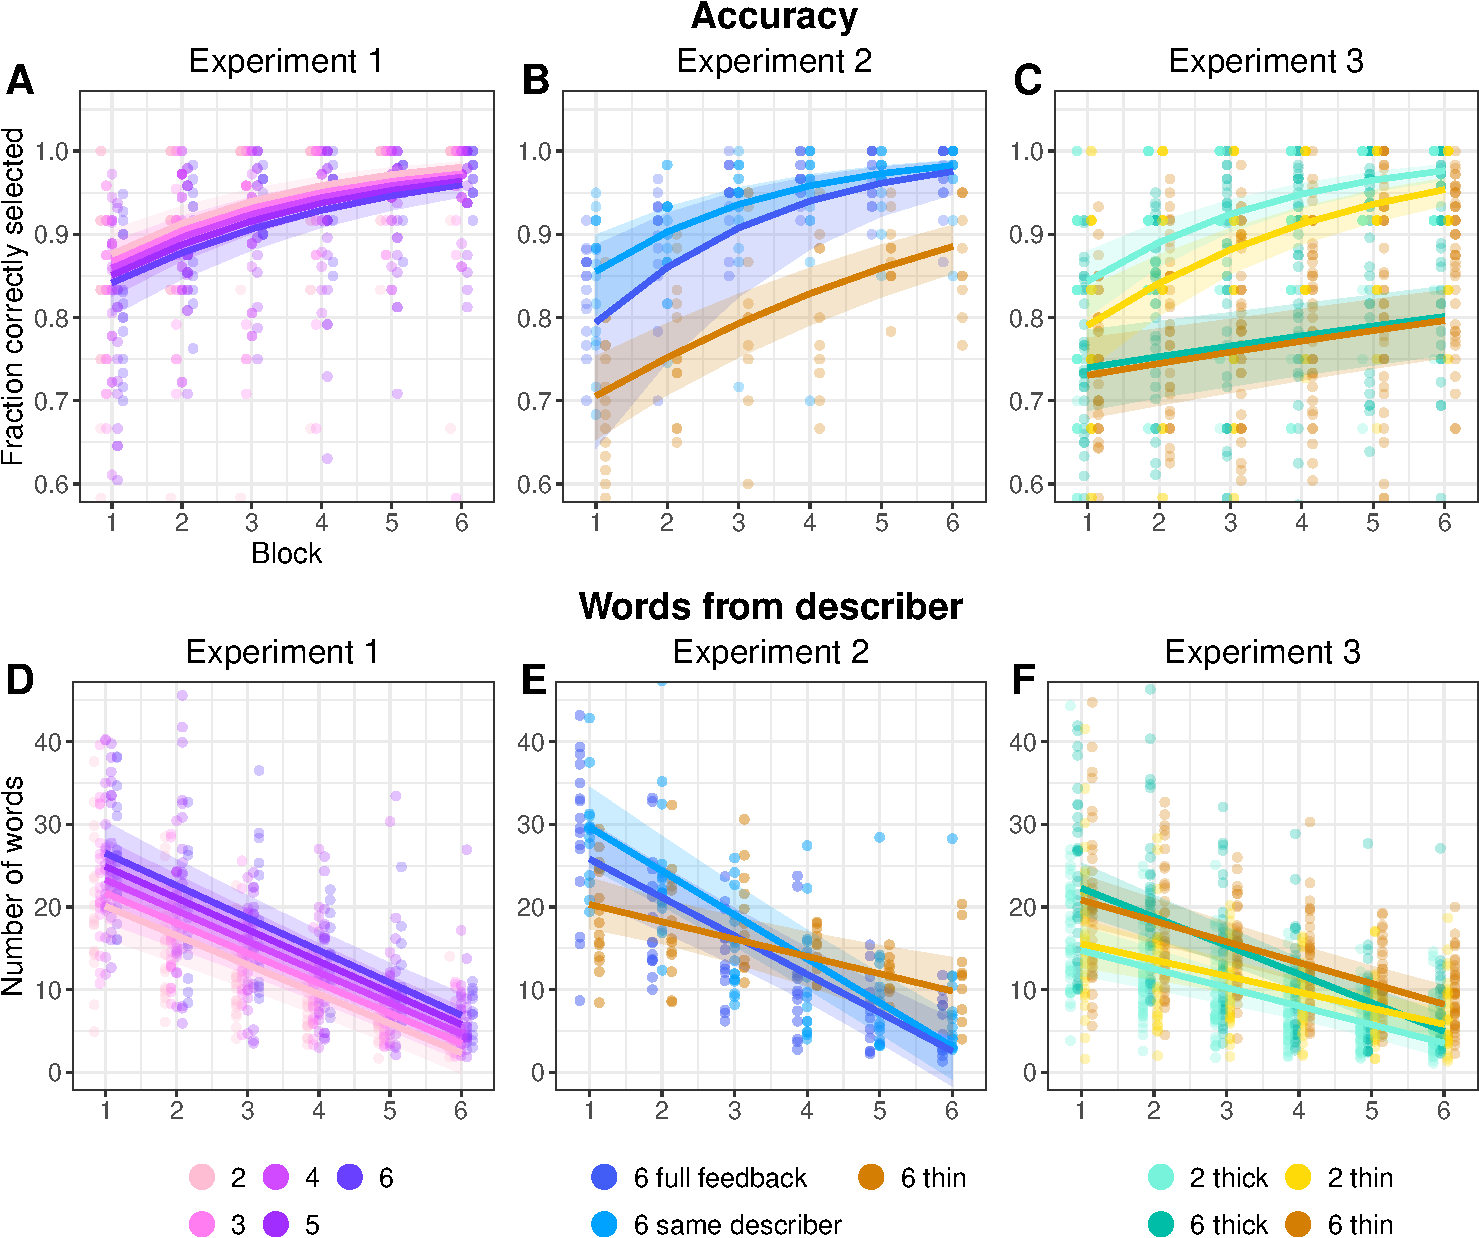
\includegraphics[width=1\linewidth]{behavioral-1.pdf} 

}

\caption{Behavioral results across all three experiments. (A-C). Matcher accuracy at selecting the target image. (D-F). Number of words produced by the describer each trial. For all, small dots are per game, per block means, and smooth lines are predictions from model fixed effects with 95\% credible intervals. Y-axes are truncated, and a few outliers points are not visible.}
\end{figure*}

\subsubsection*{Smaller and higher-coherence groups are more
accurate}\label{smaller-and-higher-coherence-groups-are-more-accurate}
\addcontentsline{toc}{subsubsection}{Smaller and higher-coherence groups
are more accurate}

Our first set of hypotheses focused on group performance: how accurately
and efficiently groups were able to perform the referential task. We
characterize group performance along two complementary metrics: (1)
matcher accuracy and (2) describer efficiency. Matcher accuracy is given
by the percent of matchers on each trial who successfully selected the
target referent. Describer efficiency is given by the number of words
produced by the describer to achieve that degree of matcher accuracy in
the group. The degree to which describers are able to communicate more
efficiently without negatively impacting matcher accuracy is indicative
of convergence on a more effective shared communication protocol within
the group.

We begin by examining matcher accuracy, the extent to which the intended
target was reliably transmitted to all matchers. We constructed a series
of 5 logistic mixed-effects regression models predicting accuracy as a
function of condition and repetition block (separate models were run for
experiment 1, each condition in experiment 2, and experiment 3). For
this and other effects, there was substantial variation at the tangram
and game levels, with some tangrams being markedly easier than others
and some groups performing differently than others. This wide variation
made it difficult to precisely estimate population-level main effects,
leading to wide credible intervals. See Figure S11 for a visualization
of the relative magnitudes of population effects and game and tangram
level variations.

Across all conditions, we observed strong positive effects of repetition
block, indicating improved performance over time (Figure
2A-C, Tables S4-S8). In Experiment 3, larger games
began with lower initial accuracy
(\(\beta=-0.64,\:95\%\:\mathrm{CrI}=[-1.05, -0.25]\)) and improved more
slowly (\(\beta=-0.34,\:95\%\:\mathrm{CrI}=[-0.43, -0.25]\)) than
smaller games, although group size differences were not reliable in
Experiment 1 (Table S4), and these experiment 3 differences were not
robust in a sensitivity analysis (Figure S4C and Table S58). Among
large groups in Experiment 2, accuracy was higher in the thicker
conditions than in the condition with thin interaction structure (Tables S5-S7), although effects of game thickness were not reliable in
Experiment 3 (Table S8).

Because each experiment only explored a slice of the full parameter
space, we also considered an exploratory analysis that pooled data
across experiments, aiming to mitigate the loss in power from running
entirely separate regression models. Specifically, we aggregated data
from all experiments into a post-hoc mega-analytic model predicting
accuracy as a function of repetition block, game thickness (thin v.
not-thin) and game size. Overall, we found evidence that accuracy
increased over time (\(\beta=0.46,\:95\%\:\mathrm{CrI}=[0.4, 0.52]\))
but the rate of increase was reduced for thin games
(\(\beta=-0.12,\:95\%\:\mathrm{CrI}=[-0.21, -0.02]\)) and larger games
(\(\beta=-0.07,\:95\%\:\mathrm{CrI}=[-0.09, -0.05]\)) compared to
smaller or thicker games. That is, smaller groups and groups with higher
coherence tended to be more accurate, though the magnitude and
reliability of these effects varied across individual experiments.

\subsubsection*{Smaller and higher-coherence groups are more
efficient}\label{smaller-and-higher-coherence-groups-are-more-efficient}
\addcontentsline{toc}{subsubsection}{Smaller and higher-coherence groups
are more efficient}

After establishing that groups were able to communicate accurately, we
turned to the challenges faced by describers when deciding how much
information to provide. Specifically, we predicted that larger and more
heterogeneous groups may initially require more information, but that
thicker interaction structure may similarly allow describers to
communicate more effectively over time. We tested these predictions
using linear mixed-effects models predicting the number of words a
describer produced on each trial as a function of condition and block.
These models counted all words the describer produced, including after
matcher contributions (similar effects were found in models predicting
the length of describer's utterances before any matcher contributions,
see Tables S21-S24).

First, as predicted, describers in larger groups produced longer
descriptions at the outset than describers in smaller groups (Figure
2D-F). This effect held for the continuous
manipulation of group size for Experiment 1
(\(\beta=1.6,\:95\%\:\mathrm{CrI}=[0.62, 2.6]\)) as well as the 2-person
versus 6-person manipulation in Experiment 3
(\(\beta=7.51,\:95\%\:\mathrm{CrI}=[3.63, 11.3]\)). Smaller groups also
continued to use shorter descriptions than larger groups over the course
of the game. In Experiment 1, the rate at which efficiency increased was
similar across different size groups
(\(\beta=-0.09,\:95\%\:\mathrm{CrI}=[-0.37, 0.18]\)). In Experiment 3,
larger groups reduced faster than smaller ones
(\(\beta=-1.22,\:95\%\:\mathrm{CrI}=[-2.06, -0.29]\)), but the faster
reduction did not fully make up for the longer initial starting point,
and was not robust to a sensitivity analysis (Figure S4F and Table
S63).

While thin 6-person games showed a flatter reduction trajectory than
thicker 6-person games in Experiment 2 (Tables S10-S12), there was no
reliable effect of game thickness on reduction in Experiment 3 (Table
S13).

The reduction patterns of description lengths is paralleled by how long
matchers took to make selections; across conditions, matchers selected
faster in later conditions (Figure S9), and the correlation between
speed and description length was consistent across experiments (Figure S10).

Aggregating across experiments with a mega-analytic model, however,
suggested that larger games were associated with steeper reduction
(\(\beta=-0.36,\:95\%\:\mathrm{CrI}=[-0.51, -0.2]\)) from a more verbose
starting point (\(\beta=2.12,\:95\%\:\mathrm{CrI}=[1.5, 2.75]\)) than
smaller games, and thin games had shallower reduction curves
(\(\beta=0.79,\:95\%\:\mathrm{CrI}=[0.04, 1.52]\)) than thicker games.
Overall, then, smaller games used shorter descriptions than larger games
across various time points in the experiment, and thinner games reduced
less than thicker games.

\begin{table}
    \centering

    \caption{Examples from 6-player groups in Experiment 3 of successful descriptions for the same image across repetitions. Describers are indicated with an asterisk. More example descriptions are in Tables S1 and S2. \\\label{listener-examples}}
    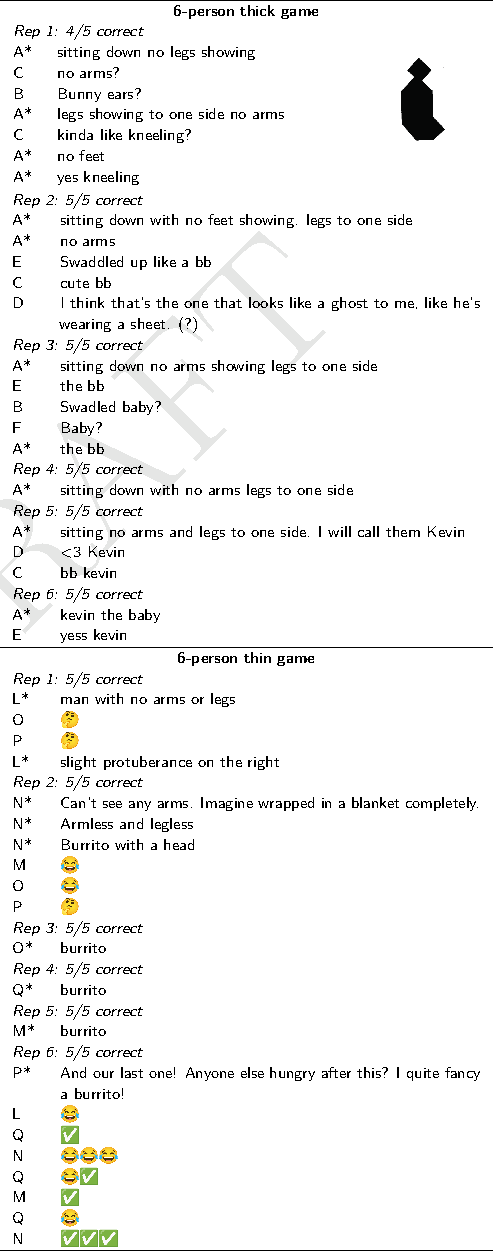
\includegraphics{table1.pdf}
%            \begin{tabular}{lp{1.9in}l}
%            	\hline
%            \multicolumn{3}{c}{\textbf{6-person thick game}}\\
%            \multicolumn{3}{l}{\textit{Rep 1: 4/5 correct}}\\
%            A*  &   sitting down no legs showing  & \multirow{5}{*} {
\includegraphics[width=.75in]{tangram_H.png}}\\                
%            C   & no arms? &\\                       
%            B  &    Bunny ears? & \\                                  
%            A*  &   legs showing to one side no arms  &\\             
%            C  &    kinda like kneeling? & \\                         
%            A*  &   no feet     & \\                                  
%            A*   &  yes kneeling  &\\
%        \end{tabular}
%        \begin{tabular}{lp{2.8in}}
%            \multicolumn{2}{l}{\textit{Rep 2: 5/5 correct}}\\
%            A*  &   sitting down with no feet showing. legs to one side \\
%            A*  &  no arms   \\                                     
%            E &      Swaddled up like a bb \\                         
%            C  &    cute bb    \\                                    
%            D  &    I think that's the one that looks like a ghost to me, like he's wearing a sheet. (?)\\
%            \multicolumn{2}{l}{\textit{Rep 3: 5/5 correct}}\\
%            A*  &    sitting down no arms showing legs to one side  \\
%            E  &   the bb   \\                                      
%            B  &  Swadled baby?  \\                                
%            F &    Baby?   \\   
%            A* &    the bb     \\ 
%            \multicolumn{2}{l}{\textit{Rep 4: 5/5 correct}}\\
%            A*    & sitting down with no arms legs to one side \\
%            \multicolumn{2}{l}{\textit{Rep 5: 5/5 correct}}\\
%            A* & sitting no arms and legs to one side. I will call them Kevin \\
%            D & <3 Kevin\\
%            C & bb kevin \\
%            \multicolumn{2}{l}{\textit{Rep 6: 5/5 correct}}\\
%      A* & kevin the baby\\
%      E & yess kevin\\
%                \hline
%       
%
%        \hline
%
%            \multicolumn{2}{c}{\textbf{6-person thin game}}\\
%            \multicolumn{2}{l}{\textit{Rep 1: 5/5 correct}}\\
%            L* & man with no arms or legs \\
%            O &      \emoji{thinking-face}\\
%            P &      \emoji{thinking-face}\\
%            L* & slight protuberance on the right \\
%            \multicolumn{2}{l}{\textit{Rep 2: 5/5 correct}}\\
%            N* &    Can't see any arms. Imagine wrapped in a blanket completely. \\
%            N* & Armless and legless \\
%            N* & Burrito with a head \\
%            M &          \emoji{face-with-tears-of-joy}\\
%            O &      \emoji{face-with-tears-of-joy}\\
%            P &              \emoji{thinking-face}\\
%            \multicolumn{2}{l}{\textit{Rep 3: 5/5 correct}}\\   
%            O* & burrito \\
%            \multicolumn{2}{l}{\textit{Rep 4: 5/5 correct}}\\
%            Q* & burrito \\
%            \multicolumn{2}{l}{\textit{Rep 5: 5/5 correct}}\\
%            M* & burrito\\
%                        \multicolumn{2}{l}{\textit{Rep 6: 5/5 correct}}\\
%            P* & And our last one! Anyone else hungry after this? I quite fancy a burrito!\\
%            L & \emoji{face-with-tears-of-joy}\\
%            Q & \emoji{check-mark-button}\\
%            N & \emoji{face-with-tears-of-joy}\emoji{face-with-tears-of-joy}\emoji{face-with-tears-of-joy}\\
%            Q & \emoji{face-with-tears-of-joy}\emoji{check-mark-button}\\
%            M & \emoji{check-mark-button}\\
%            Q & \emoji{face-with-tears-of-joy}\\
%            N & \emoji{check-mark-button}\emoji{check-mark-button}\emoji{check-mark-button}\\
%                        \hline
%        \end{tabular}
%    %\end{subtable}
\end{table}

\subsubsection*{Larger groups make greater use of matcher
contributions}\label{larger-groups-make-greater-use-of-matcher-contributions}
\addcontentsline{toc}{subsubsection}{Larger groups make greater use of
matcher contributions}

As a final measure of group performance, we examined the back-and-forth
interactions between the describer and the group of matchers. Matchers
use their chat contributions to actively provide feedback, ask
questions, offer alternative descriptions, and seek clarification about
the describer's referring expressions. Example transcripts from
successful games, one in the 6-thick condition and one in the 6-thin
condition, are shown in Table \ref{listener-examples}. Additional
examples are in Tables S1 and S2. Overall, we found that larger
groups displayed a higher proportion of trials where at least one
matcher produced utterances (Figure S6A,
\(\beta=0.79,\:95\%\:\mathrm{CrI}=[0.58, 0.98]\)), which declined across
repetition blocks (\(\beta=-0.8,\:95\%\:\mathrm{CrI}=[-0.97, -0.62]\)).
On an individual level, a matcher in a larger group was more likely to
make contributions than a matcher in a smaller group, although each
contribution tended to be shorter (Figure S7, Tables S18 and S20). The
length of matcher interjections also decreased over time, especially for
large groups (Figure S6D,
\(\beta=-0.41,\:95\%\:\mathrm{CrI}=[-0.72, -0.11]\)) consistent with the
need for early matcher involvement in establishing referential
conventions. Emoji use in Experiment 3 followed similar trends (Figure S8). Overall, describers in larger groups receive more total input
from matchers, suggesting larger groups may require greater
participation by matchers to reliably establish common ground.

\subsubsection*{Descriptions converge faster in groups with thicker
channels}\label{descriptions-converge-faster-in-groups-with-thicker-channels}
\addcontentsline{toc}{subsubsection}{Descriptions converge faster in
groups with thicker channels}

\begin{figure*}[t!]

{\centering 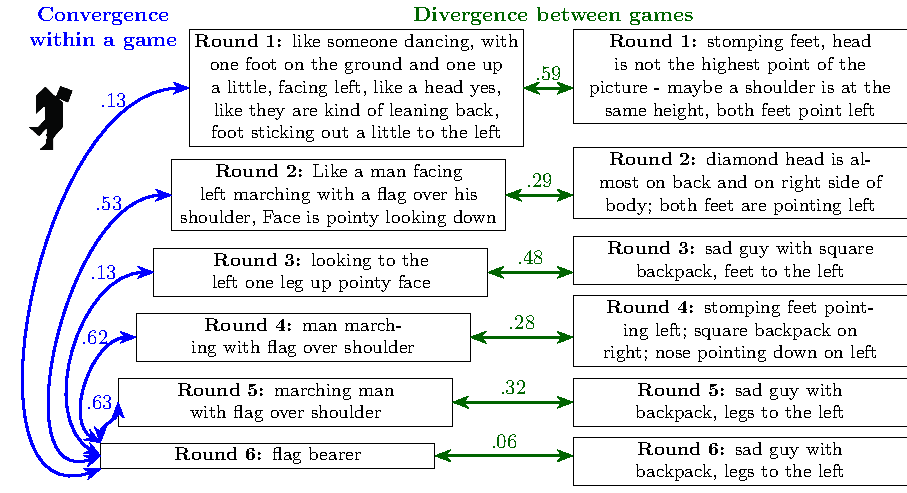
\includegraphics[width=1\linewidth]{sbert.pdf} 

}

\caption{Example utterances describing the shown tangram figure produced by two 3-player games in Experiment 1. To measure convergence within a game (blue), we measured the cosine similarity between SBERT embeddings of descriptions and the embedding of the round 6 utterance (taken to be the convention). Higher cosine similarity indicates more similar meaning. To measure divergence between games (green), we measured the similarity between embeddings of utterances from the same round across games.}
\end{figure*}

In the previous sections, we examined three metrics of communicative
performance in groups of different sizes and interaction structures. We
confirmed that groups in all conditions replicated the classic patterns
of increasing accuracy and decreasing description length. We also found
some initial evidence that larger groups may struggle to improve
performance in the absence of thick communication channels. Here, we aim
to better understand the mechanisms that allow describers to use shorter
descriptions without sacrificing accuracy. In particular, we explore the
hypothesis that interaction structure and group size affect performance
through a \emph{convention formation} process (37). Under a recent model
of convention formation (40), groups are able to leverage their shared
history to coordinate on stable expectations about how to refer to
particular images. This model makes specific predictions about how
interaction structure affects the ability to coordinate, in terms of the
available feedback.

First, due to heterogeneity in the group -- 6 individuals who may have
diverging conceptualizations --- a rational describer should provide a
strictly more detailed initial description to hedge against multiple
possible misunderstandings, as we previously observed. Second, all
groups should display the characteristic dynamics of conventions:
\emph{stability}, or convergence within group, and \emph{arbitrariness},
or divergence to multiple equilibria across groups. Third, convergence
should be faster when a single individual is consistently in the
describer role and when matchers are able to freely respond in natural
language, as describers are able to aggregate feedback about the
effectiveness of their own utterances from block to block and also
immediately correct specific misunderstandings within a given trial.

To assess the dynamics of describer descriptions, we examine the
\emph{semantic similarity} of descriptions within and across games. We
quantified description similarity by concatenating describer messages
together within a trial and embedding this description into a
high-dimensional vector space using SBERT. SBERT is a BERT-based
sentence embedder designed to map semantically similar sentences to
embeddings that are nearby in embedding space. Semantically meaningful
comparisons between sentences are made by taking pairwise cosine
similarities between the embeddings (46).

To measure stability, or convergence within groups, we compared
utterances from blocks one through five to the final (block six)
description for the same image from the same game. To measure
arbitrariness, or divergence across groups depending on group-specific
history, we compared utterances produced by different describers for the
same image in the corresponding blocks. Figure 3
illustrates these two measures with example utterances and their
within-game and between-game cosine similarities.

\begin{figure*}[t!]

{\centering 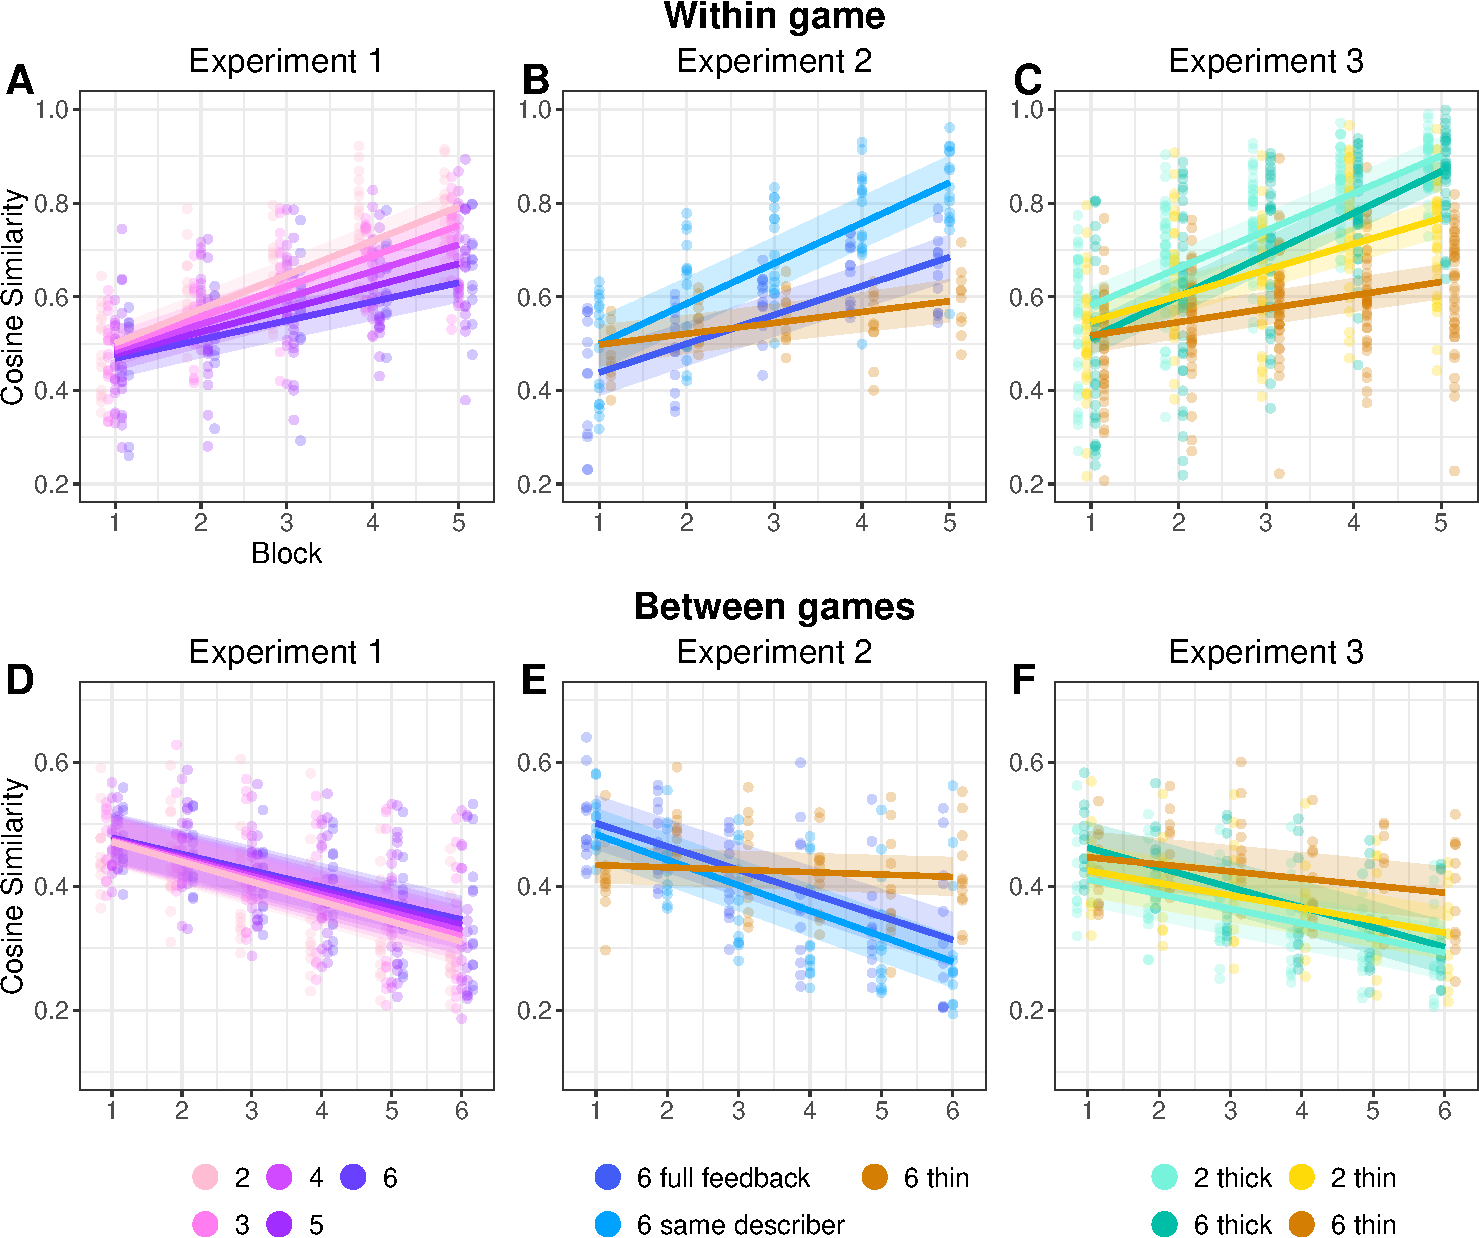
\includegraphics[width=1\linewidth]{sbert-1.pdf} 

}

\caption{Language similarity results measured with pairwise cosine similarity between embeddings of two utterances. (A-C). Convergence of descriptions within games as measured by similarity between an utterance from block 1-5 to the block 6 utterance in the same game for the same image. (D-F). Divergence of descriptions across games as measured by the similarity between two utterances produced for the same image by different groups in the same block. For all, small dots are per game, per block means, and smooth lines are predictions from model fixed effects with 95\% credible intervals. Y-axes are truncated, and a few outliers points are not visible.}
\end{figure*}

We modeled semantic convergence with a mixed effects linear regression
model predicting the similarity between a block 1-5 utterance and the
corresponding block 6 utterance as a function of the earlier block
number and condition (Figure 4A-C; Tables S25-S29). All
conditions showed some convergence toward a conventional ``shorthand''
for the picture, but the speed of convergence was affected both by group
size and channel width. First, we found that smaller groups reached
stable descriptions faster than larger games. In Experiment 1, initial
similarity was invariant across group size
(\(\beta=-0.008,\:95\%\:\mathrm{CrI}=[-0.021, 0.005]\)), but smaller
groups converged faster (Figure 4A,
\(\beta=-0.008,\:95\%\:\mathrm{CrI}=[-0.011, -0.005]\)). In Experiment
3, 6-person thick games started off further from their eventual
convention than 2-person thick games
(\(\beta=-0.069,\:95\%\:\mathrm{CrI}=[-0.113, -0.025]\)) but closed the
gap over time (Figure 4C,
\(\beta=0.009,\:95\%\:\mathrm{CrI}=[0.001, 0.017]\), this effect was not
robust to sensitivity analysis, Figure S5C and Table S68). Second,
thicker games tended to converge faster than thin games (Figure
4B-C). In Experiment 3, small thin games started off
slightly further from their convention than small thick games, and this
gap widened over time
(\(\beta=-0.025,\:95\%\:\mathrm{CrI}=[-0.033, -0.017]\)). Finally, the
combination of thin interaction structure and larger group hindered
convergence more than either factor individually. Beyond the generally
slower convergence in thin games, 6-person thin games showed
substantially slower convergence even compared to 2-person thin games in
Experiment 3 (\(\beta=-0.035,\:95\%\:\mathrm{CrI}=[-0.047, -0.025]\)).

Pooling across experiments in a mega-analysis confirms this pattern.
Thin games converge less than thick games overall
(\(\beta=-0.016,\:95\%\:\mathrm{CrI}=[-0.025, -0.008]\)), and
\emph{large} thin games are especially slow to converge
(\(\beta=-0.007,\:95\%\:\mathrm{CrI}=[-0.01, -0.004]\)). Across games,
convergence towards the last utterance was driven by cumulative
increasing similarity between pairs of utterances in adjacent blocks (Figure S12D-F, Tables S40-S44). In early rounds, descriptions could
change substantially between rounds, but by later rounds, many
descriptions had already reduced and solidified and varied little round
to round. In summary, we found that stable descriptions emerged earlier
if the group was smaller, or if the group had a thick interaction
structure.

\subsubsection*{Games with thicker channels diverge from one another
more
quickly}\label{games-with-thicker-channels-diverge-from-one-another-more-quickly}
\addcontentsline{toc}{subsubsection}{Games with thicker channels diverge
from one another more quickly}

While groups may initially overlap in their descriptions, including
details of shapes or body parts, we predicted that their descriptions
would become increasingly dissimilar as groups increasingly adapt to
their own idiosyncratic shared history. To test this effect, we
constructed a mixed-effects linear regression model predicting the
cross-game similarity between a pair of utterances for the same image. A
decrease in the similarity between different groups descriptions
occurred in every condition, indicating increasing arbitrariness and
group-specificity of descriptions (Figure 4D-F, Tables
S30-S34). However, different game sizes and interaction structures
revealed very different strengths of divergence.

First, smaller games used more group-specific language. In Experiment 1,
smaller games diverged more quickly than larger games
(\(\beta=0.001,\:95\%\:\mathrm{CrI}=[0.001, 0.002]\)). In Experiment 3,
2-person thick games started off more dissimiliar than 6-person thick
games, although 6-person games diverged faster and eventually approached
the dissimilarity levels of 2-person thick games (Table S34). Second,
thicker interaction structure was associated with stronger
group-specific divergence. In Experiment 3, 2-person thin games diverged
more slowly than 2-person thick games
(\(\beta=0.004,\:95\%\:\mathrm{CrI}=[0.002, 0.005]\)). As with the
convergence patterns, large games with thin interaction structures had
the flattest trajectories, as thinness and largeness compounded. In
Experiment 3, 6-person thin games diverged even less than 2-player thin
games (Figure 4F,
\(\beta=0.017,\:95\%\:\mathrm{CrI}=[0.015, 0.019]\)), and in Experiment
2, 6-person thin games barely diverged at all (Figure 4E,
\(\beta=-0.004,\:95\%\:\mathrm{CrI}=[-0.006, -0.001]\)). A mega-analytic
model confirms this pattern: thin games differentiate less between
groups (\(\beta=0.005,\:95\%\:\mathrm{CrI}=[0.004, 0.007]\)) and large
thin groups differentiate even less
(\(\beta=0.004,\:95\%\:\mathrm{CrI}=[0.004, 0.005]\)).

As a complement to the embedding analysis, we also examined the
frequency of a few classes of words in the descriptions. Literal
geometric words (ex. square, triangle, etc) and words for body parts
(leg, arm, etc) are common early in games, but decline over repetition
in most conditions, to be replaced by more abstract descriptions that do
not contain these classes of words (Figure S2). The 6-person thin
condition, however, retains a higher level of literal geometric and body
part words, along with high levels of positional words (above, left,
below, etc) and posture words (kicking, standing, seated, etc), with a
lower level of utterances that do not contain any of these classes of
words.

\section*{Discussion}\label{discussion}
\addcontentsline{toc}{section}{Discussion}

From classrooms to boardrooms, human communication often takes place in
multi-party settings. However, experimental research rarely focuses on
such settings, largely due to practical obstacles. In the current work,
we asked how convention formation processes, typically studied in dyadic
reference games, unfold in larger groups and under varying interaction
structures. Across 3 online experiments and 11 experimental conditions,
we varied multiple features of interaction structure including group
size, modality of matcher contributions, and degree of group coherence.
All conditions replicated classic dyadic phenomena: increasing accuracy
and efficiency, semantic convergence within games, and differentiation
of descriptions between groups. However, we also found that the
interaction structure substantially affects how rapidly groups develop
partner-specific conventions. Small groups may be able to successfully
form conventions under limited feedback, but larger groups require
thicker interaction structure. Multi-player groups may therefore reveal
key factors which are masked in purely dyadic settings.

Increasing efficiency, for example, has often been taken as an index of
group-specific convention formation (10, 11, 37, 47). In our work,
however, we observe distinct patterns for measures of raw utterance
length compared to the dynamics of semantic content. In Experiment 3,
thin 6-person games showed much less group-specific divergence despite
comparable accuracy and efficiency. This gap raises the possibility that
it is possible to become more efficient and accurate without negotiating
a unified group-specific label. Instead, they may be relying more
strongly on the group's priors (48). Thus, we encourage measures of
semantic content (and not just performance) when evaluating convention
formation. The transcripts for these games provide a rich dataset for
exploring different ways language is used to form referential
conventions.

The causal mechanisms driving group size effects remain unclear. There
are many differences between a 2-person group and a 6-person group that
could plausibly lead to different outcomes. For example, in a dyad,
producers can tailor their utterances to the one matcher, but in large
groups, producers must balance the competing needs of different
comprehenders (10, 20, 38). These effects likely vary with the knowledge
state and the communication channels available to comprehenders (8, 9,
13). Further work digging into the language used and the interactions
between participants might unearth plausible mechanisms for how
differences in group size and interaction structure influence outcomes,
pointing towards future experimental conditions.

Even within the boundaries of the repeated reference game paradigm,
there is a high-dimensional space of possible experiments. We sampled
only a few points along a few salient dimensions. In our experiment 3,
we grouped some factors together in order to run more games in each
condition: a fully factorial design would have been too expensive to
power adequately. We instantiated a ``thin'' channel by limiting
matchers to 4 discrete utterances (emojis), but there are other possible
restrictions that could be placed on the channel, such as rate-limited
typing or explicit time pressure. Future work could explore other
dimensions of the interaction structure, introducing pre-existing
relationships or familiarity among group members, alternative incentives
involving competition and power, or alternative referential targets
involving more complex concepts.

A particularly important dimension shaping interaction is the modality
of communication, including whether whether the participants use oral or
written language, whether they are co-present in the same space, and
whether they have visual access to each others' faces and gestures.
Distinct modalities carry distinct affordances and norms. In this work,
we relied on a text-based chat modality without allowing co-presence or
visual access.

We suspect that the general pattern of effects we see, in terms of group
size and coherence, are likely to extend to other modalities. However,
different modalities may allow for different strategies that may be more
or less sensitive to group size, describer rotation, or different levels
of matcher contributions. For instance, in face-to-face oral settings,
it may be easier for describers to continuously talk until interrupted,
or to monitor the comprehension of individual group members from their
facial expressions.

In conclusion, narrowly focusing on the settings that are easy to study
in the lab -- dyads with rich communication channels -- can lead to
theories that mispredict how interactions play out in multi-party
groups. By studying common ground and coordination across a wider range
of interaction structures, we can develop a more nuanced understanding
of the obstacles that stand in the way of successful communication and
how groups can overcome them. This understanding can inform the design
of policies and collaborative platforms that promote effective
communication in various contexts, from small-scale conversations to
large-scale civic discourse. As remote work and online communication
become increasingly prevalent, it is increasingly crucial to understand
how the structure of group communication environments shapes the
effectiveness of human communication.

\matmethods{

Our iterated reference task was implemented with Empirica (42), a
React-based web development framework for real-time multi-player tasks.
Our experiments were designed sequentially and pre-registered
individually.\footnote{Experiment 1: \url{https://osf.io/cn9f4} for the
  2-4 player groups, and \url{https://osf.io/rpz67} for the 5-6 player
  data run later. Experiment 2: same describer at
  \url{https://osf.io/f9xyd}, full feedback at
  \url{https://osf.io/j5zbm}, and thin at \url{https://osf.io/k5f4t}.
  Experiment 3: \url{https://osf.io/untzy}} We followed the
pre-registered analysis plan for each experiment, although accuracy
models were not explicitly specified until Experiment 3, and linguistic
analyses were only verbally described starting with Experiment 2b.
Results from some pre-registered models are omitted from the main text
for brevity but are shown in the SI. Exploratory mega-analytic models
pooling across the three experiments were not pre-registered.

All materials, data, and analysis code is available at
\url{https://github.com/vboyce/multiparty-tangrams}.

\subsubsection*{Participants}\label{participants}
\addcontentsline{toc}{subsubsection}{Participants}

This research was reviewed and deemed exempt by the Stanford IRB under
protocol 20009 ``Online investigations of language learning''. All
participants gave their informed consent before participating in the
experiments. Participants were
recruited using the Prolific platform. All participants self-reported as
fluent native English speakers on Prolific's demographic prescreen.
Experiment 1 took place between May and July 2021, Experiment 2 between
March and August 2022, and Experiment 3 in October 2022. Each
participant took part in only one experiment and was blocked from
participating in subsequent experiments. As games with more participants
tended to run longer, we paid participants different rates based on
group size, with the goal of a consistent \$10 hourly rate. Participants
were paid \$7 for 2-player games, \$8.50 for 3-player games, \$10 for
4-player games, and \$11 for 5- and 6-player games. When one player
occupied the describer role for the entirety of a 6-player game, they
were rewarded an additional \$2 bonus. Across all games, participants
could earn up to \$2.88 in performance bonuses.

A total of 1319 people participated across the 3 experiments. We
recruited enough participants for 20 games in each condition in
experiments 1 and 2 and 40 games per condition in experiment 3. However,
due to attrition in filling the games initially and due to participants
dropping out of the games, we ended up with fewer games in some
conditions. For logistical reasons of matching participants into
real-time games, we had to recruit participants in fairly large batches,
and so did not have precise control to add new games to replace games
that did not fill or had participants drop out early. A breakdown of
number of games and participants in each condition is shown in Table
S3 along with further discussion of recruitment logistics.

\subsubsection*{Materials}\label{materials}
\addcontentsline{toc}{subsubsection}{Materials}

The same 12 tangram images, drawn from (44) and (37), were used every
block. These images were displayed in a 4 \(\times\) 3 grid with the
order randomized across participants to disincentivize spatial
descriptions such as ``top left,'' as the image might be in a different
place on the describer's and matchers' screens. To reduce cognitive load
from visual search, the locations were fixed for each participant across
trials.

\subsubsection*{Procedure}\label{procedure}
\addcontentsline{toc}{subsubsection}{Procedure}

The experimental procedure was very similar across the three
experiments. We first describe the procedure used in Experiment 1 and
then describe the differences in later experiments.

\paragraph{Experiment 1}

Participants were directed from Prolific to our custom web application,
where they were presented with a consent form and a series of
instruction pages explaining the protocol. After finishing the
instructions, they needed to pass a quiz to proceed. They were then
directed to a ``waiting room'' lobby. Once the lobby filled to the
required number of players, the game began. One lobby was filled before
another was started; if a participant was waiting for 5 minutes, that
lobby timed out, and the participant was paid without completing the
experiment. Due to technical constraints with assigning participants to
lobbies and games, only games of a single experimental condition could
be active at a time. Thus, different conditions were run on different
days or times of day.\\
One of the participants was randomly selected to begin in the role of
describer, and the other participants were assigned to the role of
matchers. On each trial, the describer saw a fixed array of tangrams
with one tangram (privately) highlighted as the \emph{target}. They were
given a chat interface to communicate the target to the matchers, who
were asked to determine which of the 12 images was the referential
target. All participants were free to use the chat box to communicate at
any time, but matchers could only make a selection after the describer
had sent a message. Once a matcher clicked, they could not change their
selection. There was no signal to the describer or other matchers about
who had already made a selection. We recorded what all participants said
in the chat, as well as who selected which image and how long they took
to make their selections.

Once all matchers had made a selection (or a 3-minute timer ran out),
participants were given feedback and proceeded to the next trial.
Matchers only received \emph{binary} feedback about whether they had
chosen correctly or not; that is, matchers who made an incorrect choice
were not shown the correct answer (see Figure S1 for example
feedback). The describer saw which tangram each matcher selected, but
matchers did not see one another's selections. Matchers got 4 points for
each correct answer; the describer got points equal to the average of
the matchers' points. These points were translated into performance
bonuses at the end of the experiment (1 point = 1 cent bonus). After the
describer had described each of the 12 images as targets, in a
randomized sequence, the process repeated with the same set of targets,
for a total of 6 such repetition blocks (72 trials).

The same person was the describer for an entire block, but participants
rotated roles between blocks. Thus, over the course of the 6 blocks,
participants were describers 3 times in 2-player games, twice in
3-player games, once or twice in 4 and 5-player games, and once in
6-player games. Rotating the describer was chosen in this first
experiment to keep participants more equally engaged (the describer role
is more work), and to provide a more robust test of our hypotheses
regarding efficiency and convention formation. After the game finished,
participants were given a survey asking for optional demographic
information and feedback on their experience with the game.

If a participant disconnected from the experiment, the game would stop.

\paragraph{Experiment 2}

Experiment 2 consisted of three different variations on Experiment 1,
all conducted in 6-player games. Each of these conditions differed from
the Experiment 1 baseline in exactly one way. In the \emph{same
describer} condition, one person was designated the describer for the
entire game, rather than having the describer role rotate. In the
\emph{full feedback} condition, all participants were shown what all
others had selected as well as the identity of the correct target. This
condition was similar to previous dyadic work, such as (44), where the
correct answer was indicated during feedback. In the \emph{thin}
condition, we altered the chatbox interface for matchers. Instead of a
textbox, matchers had 4 buttons, each of which sent a different emoji to
the chat. Matchers were given suggested meanings for the 4 emojis during
the instruction phase. They could send as many emojis as desired; for
instance, they might initially indicate confusion, and later indicate
understanding. In addition, for the thin condition, we added
notifications that appeared in the chat box marking the time when each
player had made a selection.

\paragraph{Experiment 3}

The thin channel condition in Experiment 3 was the same as the thin
condition in Experiment 2. The thick condition combined the two
coherency-enhancing variations from Experiment 2: the same participant
remained in the describer role throughout, and full feedback was given
about the correct answer and what all other players had selected. Across
both conditions in Experiment 3, notifications were sent to the chat to
indicate when a participant had made a selection. For experiment 3, game
lobbies worked slightly differently, and 5 minutes after the first
participant had joined the lobby, the game started if there were at
least two participants. Correspondingly, in experiment 3, games did not
stop if a player disconnected, instead if there were at least two
players still active, the game continued, swapping a player into the
role of describer if necessary to continue the game.

\subsubsection*{Data pre-processing and
exclusions}\label{data-pre-processing-and-exclusions}
\addcontentsline{toc}{subsubsection}{Data pre-processing and exclusions}

Participants could use the chat box freely, which meant that the chat
transcript contained some non-referential language. The first author
skimmed the chat transcripts, tagging utterances that did not refer to
the current tangram. These were primarily pleasantries (``Hello''),
meta-commentary about how well the task was going, and bare
confirmations or denials (``ok'', ``got it'', ``yes'', ``no''). We
excluded these utterances from our analyses. Note that chat lines
sometimes included non-referential words in addition to words referring
to the tangrams (``ok, so it looks like a zombie'', ``yes, the one with
legs''); these lines were retained intact.

In Experiments 1 and 2, games did not start if there were not enough
participants and ended if any participant disconnected. In Experiment 3,
games started after a waiting period even if they were not entirely full
and continued even in the event that a participant disconnected (with
describer role reassigned if necessary), unless the game dropped below 2
players. The distribution of player counts in games that were initially
recruited to be 6 player games is shown in Figure S3. The realities of
online recruitment and disconnection meant that the number of games
varied between conditions. We excluded incomplete blocks from analyses,
but included complete blocks from partial games (See Table S3). When
skimming transcripts to tag non-referential utterances, we noticed that
one game in the 6-player thick condition had a describer who did not
give any sort of coherent descriptions, even with substantial matcher
prompting. We excluded this game from analyses.

\subsubsection*{Modelling strategy}\label{modelling-strategy}
\addcontentsline{toc}{subsubsection}{Modelling strategy}

We fit all regression models in brms (49) with weakly regularizing
priors. We were unable to fit the full pre-registered mixed effects
structure in a reasonable amount of time for some models, so we included
the maximal hierarchical effects that were tractable. All model results
and priors and formulae are reported in the SI. Models of accuracy used
by-group random intercepts only, models of word count used full mixed
effect structure, and models of S-BERT similarities used by-group and
by-target random intercepts as applicable (see Figure S11). Models of
matcher accuracy were logistic models with normal(0,1) priors for betas
and sd. Models of describer efficiency were run as linear models with an
intercept prior of normal(12,20), a beta prior of normal(0,10), an sd
prior of normal(0,5) and a random-effect correlation prior of lkj(1).
For all of the models of SBERT similarity, we used linear models with
the priors normal(.5,.2) for the intercept, normal(0,.1) for betas, and
normal(0,.05) for sd. As an additional post-hoc analysis, we ran
mega-analytic models combining data across all experiments. For these
models, we grouped the 3 thin-ish conditions (2c, and the two thin
conditions of experiment 3) as one level, and coded the rest of the
conditions as thick-ish. Game size was coded as a continuous measure (2
through 6). The priors for the mega-analytic models were the same as for
the per-experiment models described above.

As a sensitivity analysis, we re-ran the primary models on the subset of
the data from games that a) completed all 72 trials and b) had the full
complement of players the entire time (relevant to 6-player experiment 3
games where games could start or continue with fewer players).
Discrepancies are mentioned in the results, and these analyses are
depicted in Figures S4 and S5 and Tables S54-S73. We also needed to
decide how to handle dropout in Experiment 3, as some of the 6-player
games did not retain all 6 players for the entire game. Our decision was
to follow an intent-to-treat analysis and treat data as missing
completely at random. Note that this choice underestimates differences
between 2-player and (genuine) 6-player games by labeling some smaller
groups as 6-player groups. We do not know exactly what leads some
participants to drop out, but it is possible that some factors may be
random (ex. connection issues) and others may be correlated with
performance (ex. frustration because group is struggling).\\
We do not know whether groups that start and continue at the full size
differ from games where some participants drop out. This is potentially
an issue across all experiments; in experiments 1 and 2, groups stopped
playing if anyone dropped out, and in experiment 3 they kept playing as
a smaller group. The number of games in each condition and rates of
dropoff are shown in Table S3 and Figure S3.
}

\showmatmethods
\showacknow

\bibsplit[8]

\begin{CSLReferences}{0}{1}
	\bibitem[\citeproctext]{ref-cazden1988classroom}
	\CSLLeftMargin{1. }%
	\CSLRightInline{C. B. Cazden, \emph{Classroom discourse: The language of
			teaching and learning.} (ERIC, 1988).}
	
	\bibitem[\citeproctext]{ref-tannen2005conversational}
	\CSLLeftMargin{2. }%
	\CSLRightInline{D. Tannen, \emph{Conversational style: Analyzing talk
			among friends} (Oxford University Press, 2005).}
	
	\bibitem[\citeproctext]{ref-caplow1957organizational}
	\CSLLeftMargin{3. }%
	\CSLRightInline{T. Caplow, Organizational size. \emph{Administrative
			Science Quarterly} 484--505 (1957).}
	
	\bibitem[\citeproctext]{ref-zack1993interactivity}
	\CSLLeftMargin{4. }%
	\CSLRightInline{M. H. Zack, Interactivity and communication mode choice
		in ongoing management groups. \emph{Information Systems Research}
		\textbf{4}, 207--239 (1993).}
	
	\bibitem[\citeproctext]{ref-branigan2006}
	\CSLLeftMargin{5. }%
	\CSLRightInline{H. Branigan, Perspectives on multi-party dialogue.
		\emph{Research on Language and Computation} \textbf{4}, 153--177
		(2006).}
	
	\bibitem[\citeproctext]{ref-ginzburg2005}
	\CSLLeftMargin{6. }%
	\CSLRightInline{J. Ginzburg, R. Fernandez, Action at a distance: The
		difference between dialogue and multilogue. \emph{Proceedings of DIALOR}
		9 (2005).}
	
	\bibitem[\citeproctext]{ref-traum2004}
	\CSLLeftMargin{7. }%
	\CSLRightInline{D. Traum,
		{``\href{https://doi.org/10.1007/978-3-540-24608-4_12}{Issues in
				{Multiparty Dialogues}}''} in \emph{Advances in {Agent Communication}},
		F. Dignum, Ed. ({Springer Berlin Heidelberg}, 2004), pp. 201--211.}
	
	\bibitem[\citeproctext]{ref-horton2005}
	\CSLLeftMargin{8. }%
	\CSLRightInline{W. S. Horton, R. J. Gerrig,
		\href{https://doi.org/10.1016/j.cognition.2004.07.001}{The impact of
			memory demands on audience design during language production}.
		\emph{Cognition} \textbf{96}, 127--142 (2005).}
	
	\bibitem[\citeproctext]{ref-horton2002}
	\CSLLeftMargin{9. }%
	\CSLRightInline{W. S. Horton, R. J. Gerrig, {SpeakersÕ} experiences and
		audience design: Knowing when and knowing how to adjust utterances to
		addresseesq. \emph{Journal of Memory and Language} 18 (2002).}
	
	\bibitem[\citeproctext]{ref-yoon2018}
	\CSLLeftMargin{10. }%
	\CSLRightInline{S. O. Yoon, S. Brown-Schmidt,
		\href{https://doi.org/10.1080/0163853X.2017.1286225}{Aim {Low}:
			{Mechanisms} of {Audience Design} in {Multiparty Conversation}}.
		\emph{Discourse Processes} \textbf{55}, 566--592 (2018).}
	
	\bibitem[\citeproctext]{ref-yoon2014}
	\CSLLeftMargin{11. }%
	\CSLRightInline{S. O. Yoon, S. Brown-Schmidt,
		\href{https://doi.org/10.1037/a0036161}{Adjusting conceptual pacts in
			three-party conversation.} \emph{Journal of Experimental Psychology:
			Learning, Memory, and Cognition} \textbf{40}, 919--937 (2014).}
	
	\bibitem[\citeproctext]{ref-weber2003}
	\CSLLeftMargin{12. }%
	\CSLRightInline{R. A. Weber, C. F. Camerer, Cultural {Conflict} and
		{Merger Failure}: {An Experimental Approach}. \emph{Manag. Sci.}
		\textbf{49}, 16 (2003).}
	
	\bibitem[\citeproctext]{ref-fox-tree2013}
	\CSLLeftMargin{13. }%
	\CSLRightInline{J. E. Fox Tree, N. B. Clark,
		\href{https://doi.org/10.1080/0163853X.2013.797241}{Communicative
			{Effectiveness} of {Written Versus Spoken Feedback}}. \emph{Discourse
			Processes} \textbf{50}, 339--359 (2013).}
	
	\bibitem[\citeproctext]{ref-fay2000}
	\CSLLeftMargin{14. }%
	\CSLRightInline{N. Fay, S. Garrod, J. Carletta,
		\href{https://doi.org/10.1111/1467-9280.00292}{Group {Discussion} as
			{Interactive Dialogue} or as {Serial Monologue}: {The Influence} of
			{Group Size}}. \emph{Psychol Sci} \textbf{11}, 481--486 (2000).}
	
	\bibitem[\citeproctext]{ref-carletta1998}
	\CSLLeftMargin{15. }%
	\CSLRightInline{J. Carletta, S. Garrod, H. Fraser-Krauss,
		\href{https://doi.org/10.1177/1046496498295001}{Placement of {Authority}
			and {Communication Patterns} in {Workplace Groups}: {The Consequences}
			for {Innovation}}. \emph{Small Group Research} \textbf{29}, 531--559
		(1998).}
	
	\bibitem[\citeproctext]{ref-metzing2003}
	\CSLLeftMargin{16. }%
	\CSLRightInline{C. Metzing, S. E. Brennan,
		\href{https://doi.org/10.1016/S0749-596X(03)00028-7}{When conceptual
			pacts are broken: {Partner-specific} effects on the comprehension of
			referring expressions}. \emph{Journal of Memory and Language}
		\textbf{49}, 201--213 (2003).}
	
	\bibitem[\citeproctext]{ref-yoon2019}
	\CSLLeftMargin{17. }%
	\CSLRightInline{S. O. Yoon, S. Brown‐Schmidt,
		\href{https://doi.org/10.1111/cogs.12774}{Audience {Design} in
			{Multiparty Conversation}}. \emph{Cogn. Sci.} \textbf{43}, e12774
		(2019).}
	
	\bibitem[\citeproctext]{ref-rogers2013}
	\CSLLeftMargin{18. }%
	\CSLRightInline{S. L. Rogers, N. Fay, M. Maybery,
		\href{https://doi.org/10.1371/journal.pone.0057211}{Audience {Design}
			through {Social Interaction} during {Group Discussion}}. \emph{PLOS ONE}
		\textbf{8}, e57211 (2013).}
	
	\bibitem[\citeproctext]{ref-cohngordon}
	\CSLLeftMargin{19. }%
	\CSLRightInline{Cohn-Gordon Reuben, R. Levy, L. Bergen, The pragmatics
		of multiparty communication. (2019).}
	
	\bibitem[\citeproctext]{ref-tolins2016}
	\CSLLeftMargin{20. }%
	\CSLRightInline{J. Tolins, J. E. Fox Tree,
		\href{https://doi.org/10.1111/cogs.12278}{Overhearers {Use Addressee
				Backchannels} in {Dialog Comprehension}}. \emph{Cogn Sci} \textbf{40},
		1412--1434 (2016).}
	
	\bibitem[\citeproctext]{ref-krauss1966}
	\CSLLeftMargin{21. }%
	\CSLRightInline{R. M. Krauss, S. Weinheimer,
		\href{https://doi.org/10.1037/h0023705}{Concurrent feedback,
			confirmation, and the encoding of referents in verbal communication.}
		\emph{Journal of Personality and Social Psychology} \textbf{4}, 343--346
		(1966).}
	
	\bibitem[\citeproctext]{ref-KraussBricker67_Delay}
	\CSLLeftMargin{22. }%
	\CSLRightInline{R. M. Krauss, P. D. Bricker, Effects of transmission
		delay and access delay on the efficiency of verbal communication.
		\emph{The Journal of the Acoustical Society of America} \textbf{41},
		286--292 (1967).}
	
	\bibitem[\citeproctext]{ref-kraut1982listener}
	\CSLLeftMargin{23. }%
	\CSLRightInline{R. E. Kraut, S. H. Lewis, L. W. Swezey, Listener
		responsiveness and the coordination of conversation. \emph{Journal of
			personality and social psychology} \textbf{43}, 718 (1982).}
	
	\bibitem[\citeproctext]{ref-KraussEtAl77}
	\CSLLeftMargin{24. }%
	\CSLRightInline{R. M. Krauss, C. M. Garlock, P. D. Bricker, L. E.
		McMahon, The role of audible and visible back-channel responses in
		interpersonal communication. \emph{Journal of Personality and Social
			Psychology} \textbf{35}, 523 (1977).}
	
	\bibitem[\citeproctext]{ref-dewhirst1971influence}
	\CSLLeftMargin{25. }%
	\CSLRightInline{H. D. Dewhirst, Influence of perceived
		information-sharing norms on communication channel utilization.
		\emph{Academy of Management Journal} \textbf{14}, 305--315 (1971).}
	
	\bibitem[\citeproctext]{ref-clark2004speaking}
	\CSLLeftMargin{26. }%
	\CSLRightInline{H. H. Clark, M. A. Krych, Speaking while monitoring
		addressees for understanding. \emph{Journal of memory and language}
		\textbf{50}, 62--81 (2004).}
	
	\bibitem[\citeproctext]{ref-garrod2007foundations}
	\CSLLeftMargin{27. }%
	\CSLRightInline{S. Garrod, N. Fay, J. Lee, J. Oberlander, T. MacLeod,
		Foundations of representation: Where might graphical symbol systems come
		from? \emph{Cognitive science} \textbf{31}, 961--987 (2007).}
	
	\bibitem[\citeproctext]{ref-swaab2012communication}
	\CSLLeftMargin{28. }%
	\CSLRightInline{R. I. Swaab, A. D. Galinsky, V. Medvec, D. A. Diermeier,
		The communication orientation model: Explaining the diverse effects of
		sight, sound, and synchronicity on negotiation and group decision-making
		outcomes. \emph{Personality and Social Psychology Review} \textbf{16},
		25--53 (2012).}
	
	\bibitem[\citeproctext]{ref-hiltz1986experiments}
	\CSLLeftMargin{29. }%
	\CSLRightInline{S. R. Hiltz, K. Johnson, M. Turoff, Experiments in group
		decision making: Communication process and outcome in face-to-face
		versus computerized conferences. \emph{Human communication research}
		\textbf{13}, 225--252 (1986).}
	
	\bibitem[\citeproctext]{ref-macmillan_communication_2004}
	\CSLLeftMargin{30. }%
	\CSLRightInline{J. MacMillan, E. E. Entin, D. Serfaty,
		{``\href{https://doi.org/10.1037/10690-004}{Communication overhead:
				{The} hidden cost of team cognition.}''} in \emph{Team Cognition:
			{Understanding} the Factors That Drive Process and Performance.},
		(American Psychological Association, 2004), pp. 61--82.}
	
	\bibitem[\citeproctext]{ref-seaman1997communication}
	\CSLLeftMargin{31. }%
	\CSLRightInline{C. B. Seaman, V. R. Basili, Communication and
		organization in software development: An empirical study. \emph{IBM
			Systems Journal} \textbf{36}, 550--563 (1997).}
	
	\bibitem[\citeproctext]{ref-ahern1994effect}
	\CSLLeftMargin{32. }%
	\CSLRightInline{T. C. Ahern, The effect of interface on the structure of
		interaction in computer-mediated small-group discussion. \emph{Journal
			of Educational Computing Research} \textbf{11}, 235--250 (1994).}
	
	\bibitem[\citeproctext]{ref-parisi2005evaluating}
	\CSLLeftMargin{33. }%
	\CSLRightInline{J. A. Parisi, D. S. Brungart, Evaluating communication
		effectiveness in team collaboration in \emph{Ninth European Conference
			on Speech Communication and Technology (INTERSPEECH)}, (2005).}
	
	\bibitem[\citeproctext]{ref-Wittgenstein1953}
	\CSLLeftMargin{34. }%
	\CSLRightInline{L. Wittgenstein, \emph{Philosophical investigations}
		(Wiley-Blackwell, 1953).}
	
	\bibitem[\citeproctext]{ref-lewis1969convention}
	\CSLLeftMargin{35. }%
	\CSLRightInline{D. Lewis, \emph{Convention: A philosophical study} (John
		Wiley \& Sons, 1969).}
	
	\bibitem[\citeproctext]{ref-krauss1964}
	\CSLLeftMargin{36. }%
	\CSLRightInline{R. M. Krauss, S. Weinheimer,
		\href{https://doi.org/10.3758/BF03342817}{Changes in reference phrases
			as a function of frequency of usage in social interaction: A preliminary
			study}. \emph{Psychon Sci} \textbf{1}, 113--114 (1964).}
	
	\bibitem[\citeproctext]{ref-clark1986}
	\CSLLeftMargin{37. }%
	\CSLRightInline{H. H. Clark, D. Wilkes-Gibbs,
		\href{http://www.speech.kth.se/~edlund/bielefeld/references/clark-and-wilkes-gibbs-1986.pdf}{Referring
			as a collaborative process}. \emph{Cognition} (1986).}
	
	\bibitem[\citeproctext]{ref-schober1989}
	\CSLLeftMargin{38. }%
	\CSLRightInline{M. F. Schober, H. H. Clark,
		\href{https://doi.org/10.1016/0010-0285(89)90008-X}{Understanding by
			addressees and overhearers}. \emph{Cognitive Psychology} \textbf{21},
		211--232 (1989).}
	
	\bibitem[\citeproctext]{ref-wilkes1992coordinating}
	\CSLLeftMargin{39. }%
	\CSLRightInline{D. Wilkes-Gibbs, H. H. Clark, Coordinating beliefs in
		conversation. \emph{Journal of memory and language} \textbf{31},
		183--194 (1992).}
	
	\bibitem[\citeproctext]{ref-hawkins2023partners}
	\CSLLeftMargin{40. }%
	\CSLRightInline{R. D. Hawkins, \emph{et al.}, From partners to
		populations: A hierarchical bayesian account of coordination and
		convention. \emph{Psychological Review} \textbf{130}, 977 (2023).}
	
	\bibitem[\citeproctext]{ref-almaatouq2022}
	\CSLLeftMargin{41. }%
	\CSLRightInline{A. Almaatouq, \emph{et al.}, Beyond {Playing} 20
		{Questions} with {Nature}: {Integrative Experiment Design} in the
		{Social} and {Behavioral Sciences}. \emph{Behavioral and Brain Sciences}
		1--55 (2022). \url{https://doi.org/10.1017/S0140525X22002874}.}
	
	\bibitem[\citeproctext]{ref-almaatouq2020empirica}
	\CSLLeftMargin{42. }%
	\CSLRightInline{A. Almaatouq, \emph{et al.}, Empirica: A virtual lab for
		high-throughput macro-level experiments. \emph{Behavior Research
			Methods} \textbf{53}, 2158--2171 (2021).}
	
	\bibitem[\citeproctext]{ref-haber2019}
	\CSLLeftMargin{43. }%
	\CSLRightInline{J. Haber, \emph{et al.},
		\href{https://doi.org/10.18653/v1/P19-1184}{The {PhotoBook Dataset}:
			{Building Common Ground} through {Visually-Grounded Dialogue}} in
		\emph{Proc. 57th {Annu}. {Meet}. {Assoc}. {Comput}. {Linguist}.},
		({Association for Computational Linguistics}, 2019), pp. 1895--1910.}
	
	\bibitem[\citeproctext]{ref-hawkins2020}
	\CSLLeftMargin{44. }%
	\CSLRightInline{R. D. Hawkins, M. C. Frank, N. D. Goodman,
		\href{http://arxiv.org/abs/1912.07199}{Characterizing the dynamics of
			learning in repeated reference games}. \emph{ArXiv191207199 Cs} (2020).}
	
	\bibitem[\citeproctext]{ref-ji2022abstract}
	\CSLLeftMargin{45. }%
	\CSLRightInline{A. Ji, \emph{et al.}, Abstract visual reasoning with
		tangram shapes in \emph{Proceedings of the 2022 Conference on Empirical
			Methods in Natural Language Processing}, (2022), pp. 582--601.}
	
	\bibitem[\citeproctext]{ref-reimers2019}
	\CSLLeftMargin{46. }%
	\CSLRightInline{N. Reimers, I. Gurevych,
		\href{https://doi.org/10.48550/arXiv.1908.10084}{Sentence-{BERT}:
			{Sentence Embeddings} using {Siamese BERT-Networks}}. (2019).}
	
	\bibitem[\citeproctext]{ref-brennan1996}
	\CSLLeftMargin{47. }%
	\CSLRightInline{S. E. Brennan, H. H. Clark, Conceptual {Pacts} and
		{Lexical Choice} in {Conversation}. 12 (1996).}
	
	\bibitem[\citeproctext]{ref-guilbeault2021}
	\CSLLeftMargin{48. }%
	\CSLRightInline{D. Guilbeault, A. Baronchelli, D. Centola,
		\href{https://doi.org/10.1038/s41467-020-20037-y}{Experimental evidence
			for scale-induced category convergence across populations}. \emph{Nat
			Commun} \textbf{12}, 327 (2021).}
	
	\bibitem[\citeproctext]{ref-burkner2018}
	\CSLLeftMargin{49. }%
	\CSLRightInline{P.-C. Bürkner, Advanced bayesian multilevel modeling
		with the r package brms. \emph{The R Journal} \textbf{10}, 395--411
		(2018).}
	
\end{CSLReferences}



% Bibliography
% \bibliography{pnas-sample}

\end{document}
